\documentclass{llncs}
	\usepackage{mathtools}
	\usepackage{amsmath}
	\usepackage{algorithm2e}
	\usepackage{graphicx}
	\usepackage{setspace}

% set algorithm captions above psuedocode
\makeatletter
\renewcommand{\@algocf@capt@plain}{above} 
\makeatother

\begin{document}

\title{Simulating International Energy Security}
	\author{David Masad}
	\date{}
	\maketitle


\begin{abstract}
Energy security is placed at risk by exogenous supply shocks, in particular political crises and conflicts that disrupt resource extraction and transportation. In this paper, a computational model of the security of international crude oil supplies is described, and its output analyzed. The model consists of country agents, linked geographically and by a directed, data-derived oil trade network. Countries stochastically experience crises, with probabilities and durations drawn randomly from data-driven distributions. The effect of these crises on secure oil supplies is measured globally and by country, and the effect of conflict contagion and spare production capacity are also estimated. The model indicates that Russia, Eastern Europe, and much of the Global South are at the greatest risk of supply shocks, while American producers are at greatest risk of demand shocks. It estimates that conflict contagion decreases energy security slightly, while spare capacity has minimal effect. 
\end{abstract}

\section{Introduction}

Energy security is defined by the International Energy Agency as ``the uninterrupted availability of energy sources at an affordable price''\cite{iea_2013}. As the world's energy demand continues to expand in the face of growing scarcity, energy security is becoming increasingly critical not just to developed countries but to developing ones as well \cite{yergin_2006}. Thus, assessing the energy security of different countries is important in order to understand the overall state of the international system. Despite this, there have been few attempts to create formal models of energy security. 

Much of the analysis to date has taken a portfolio-based approach. \cite{wu_2009} uses portfolio diversity to analyze China's mix of crude oil and processed petroleum products. The paper notes that ``Oil import-specific risk derives from events, such as political events, natural disaster and so on, that are not related to general movements in the international market'', but does not analyze the risks of such events directly. It does, however, address the relatively less significant risk of piracy along several shipping routes. \cite{stirling_2010} and \cite{skea_2010} take a broader, more theoretical approach, and develops a multicriteria methodology for evaluating the diversity of an entire energy portfolio as it contributes to energy security. However, changing the composition of an entire energy portfolio takes a great deal of time -- it is a long-term process, measured in years or decades. Similarly, \cite{jacobson_2009} evaluates a set of possible future courses of action to jointly address climate, environmental and energy-security concerns -- again, courses of actions only implementable over the long term.

Short-term energy security, in contrast, appears to have been little-addressed in the literature. However, an important short-term analysis, MOSES (Model of Short-term Energy Security), was created within the International Energy Agency (IEA), the intergovernmental organization of the world's major oil importers established in part to protect their energy security. As the name of the model indicates, MOSES focuses on short-term risks, which it defines as a timescale of days and weeks. Furthermore, MOSES assigns risk scores based on a broad but ultimately static set of indicators. In particular, the indicator used to measure political stability is the ``weighted average of political stability of suppliers''. However, the greater the diversity of suppliers (another input into the model), the greater the potential range of political stabilities. Averaging ratings of political risk eliminates the complexity that characterizes international political systems \cite{cederman_1997,geller_2011}, and ignores the possibility of crisis and conflict contagion \cite{black_2013}, by which conflict in one place can trigger other conflicts nearby. 

In fact, as \cite{hamilton_2003} describes, oil supply shocks have been driven caused by conflict involving oil producers, both domestic and international. \cite{hamilton_2003} argues that supply shock-driven changes to oil prices have a nonlinear effect on GDP, while \cite{kilian_2008} argues that the macroeconomic effects of the oil shocks themselves are small. Nevertheless, the price of oil is only an indirect indicator of energy security; if a substantial volume of oil cannot be extracted or exported, and hence is unavailable for consumption, it poses an energy security risk regardless of what the price of oil is doing. 

In this paper, I present a novel model linking energy security with political instability. At the core of the model is the supply and demand for crude oil at the country level, both imported and domestically-produced. Supply and demand are placed at risk when countries experience crises and conflicts. The model operates on the meso timescale, of months and years rather than days or decades.  It produces country-level and global time-series of oil security indicators with each iteration. By running multiple iterations with different parameters, I generate notional near-future scenarios of changes in international energy security. 

The model is designed to be `as simple as possible, but no simpler.'  As such, it straddles the boundary between a complicated cellular automata on a network and a simple agent-based model. As we shall see, at its simplest configuration, the model is essentially stochastically sampling from the space of possible international crisis configurations and measuring their impact, with no agent decisionmaking. By incrementally adding elements (in particular, the possibility of conflict contagion and rapid increases of production to counterbalance supply shocks), we can estimate the impact of the additional complexity. 

In the remainder of the paper, I describe the model in more detail, its data sources, and its various submodels. I use the model to conduct several experiments, describe the output, and conduct a sensitivity analysis. Finally, I discuss my conclusions, both regarding international energy security and the challenges and opportunities of this type of modeling.

\section{Model Description}

\subsection{Overview}

The model consists of countries, each of which has a set supply of and demand for crude oil. Countries are linked geographically, and by a network of export-import relationships. Each month, some countries enter crisis at random; the exports and imports of countries in crisis are considered \emph{at risk}. If \textbf{Contagion} is enabled, a crisis in one country may spread to its immediate geographic neighbors. If \textbf{Assistance} is enabled, oil exporters may increase their production to balance a loss of secure oil by their major import partners.

The model parameters currently remain fixed for each run: political instability, supply, demand, and trade relations are treated as constant. 

\subsection{Data Sources}
The model inputs are empirical whenever possible. Data inputs are oil trade relationships, country political instability,  country consumption of domestic oil production, and spare production capacity.

The network of oil imports and exports comes from the United Nations-maintained COMTRADE database \cite{un_2013}. I extract all imports of crude petroleum (product code 2709) and other unprocessed petroleum (product code 2710) for 2012, the most recent year for which complete data is available. Note that import data appears to be more reliable than export data: many major oil producers (particularly Saudi Arabia and Venezuela) only report export volume by region (e.g. Europe, North America); however, the majority of their trade partners report their imports from them.

For the majority of countries, I assume that supply and demand are equal to total export and imports, respectively. For the top ten oil producers, I use US Energy Information Administration (EIA) estimates \cite{eia_2013}, country estimates \cite{canada_2009,eia_domestic}, expert reports \cite{mohamedi_2010}, and media sources \cite{rasmi_2013} for those countries' consumption of their own domestic production. 

Spare capacity is particularly difficult to estimate, and varies over time based on the price of oil and other factors \cite{mearns_2012}. I use media sources such as \cite{daya_2012} and subject-matter expert (SME) analysis such as \cite{mearns_2012} in order to estimate the spare capacity of other countries, when possible. I also assign a default spare capacity of 10\% based on SME input.

Political instability estimates are taken from the Economist Intelligence Unit's Political Index ratings \cite{eiu_2013}. These are in turn estimated based on the methodology developed by the Political Instability Task Force \cite{goldstone_2005}, which could predict the onset of internal instability in a two-year period with 80\% accuracy. Thus, these scores are normalized such that a rating of 10 (the maximum) is associated with an approximately 80\% probability of instability within a 24-month timeframe, translating into a 6.5\% monthly probability of crisis onset.

Crisis duration is drawn independently from onset. \cite{cioffi_2004} and others have argued that internal and external conflict durations follow a power law distribution, which I use here. I calibrate the power law coefficient from two datasets: the UCDP/PRIO Armed Conflict Dataset \cite{lotta_2013} for military conflicts, and the Social Conflict in Africa Database \cite{hendrix_2013}, which includes both armed and lower-level social conflicts. I subset the PRIO dataset for conflicts in Africa and merge it with SCAD, eliminating duplicates and events below the severity of a general strike, in order to obtain as complete as possible a set of crises and conflicts that may be associated with an oil production  shock. I find the duration of each event in months, and fit a power law to the resulting distribution, resulting in an estimated coefficient of $\mathbf{-1.37}$.

\subsection{Formal Description}

The model consists of \textbf{Country} agents, possessing several characteristics and linked by two networks: a directed \textbf{trade network}, and an undirected \textbf{geographic adjacency} network, where the country agents are the network nodes.

Model variables may be \emph{fixed} based on data, \emph{parameters} that are fixed for each run and may be changed between them, or \emph{states} of the agents and edges that vary during the model.

The model was written in Java, using the MASON package \cite{luke_2005}, with additional analysis done in Python. 

\subsubsection{Networks}

Agents are connected by two networks, which we can also express as matrices. Let $\mathbf{G}$ be the geographic adjacency matrix, such that $g_{i,j}=g_{j,i}=1$ when counties $i$ and $j$ are geographically contiguous or near-contiguous, and $0$ otherwise. 

Let $\mathbf{E}$ be the trade matrix, such that $e_{i,j}$ denotes the volume of oil exports from $i$ to $j$. Note that if the assistance submodel is turned on, the values of $\mathbf{E}$ may change over time.

\subsubsection{Agent parameters and variables}

Each agent represents an independent country. Agents are associated with the \textbf{geometry} of their position on a world map, which determines their neighbors. They are described by two submodels: an oil model, and a crisis model.

\paragraph{Oil Submodel}
\begin{itemize}
	\item \textbf{Domestic Share} of the country's oil demand satisfied by domestic production. For most countries, this defaults to 0; for the top ten oil producers, it is set based on US Energy Information Administration data \cite{eia_2013}.
	\item \textbf{Total Imports} is the sum of the current volume of all oil imports. 
	\item \textbf{Total Demand} is the sum of current imported and domestic oil consumed. Since the EIA reports the share of total consumption that is domestically-sourced, demand is calculated as: $$\text{Total Demand}_i = \sum_j e_{j,i} \cdot (1 - \text{Domestic Share})^{-1}$$
	With $Total Imports$ set at the initial baseline. If current imports increase (as explained below) then supply will exceed demand. 
	\item \textbf{Total Exports} is the sum of current exported oil to all other countries.
\end{itemize}

\paragraph{Crisis Submodel}
\begin{itemize}
	\item \textbf{Instability} is a measure of the country's political instability on a 0-10 scale, and determines the probability of a crisis or conflict -- a production shock. It is obtained from \cite{eiu_2013}. 
	\item \textbf{In Crisis} is simply a boolean variable determining whether or not a country is currently experiencing a crisis or conflict.
	\item \textbf{Crisis Length} is the number of months remaining in a crisis, if one is currently in process. When a country enters crisis, this number is drawn from a power law distribution. Specifically, in order to accommodate the limitations of the MASON random-number generator, I use a uniform approximation \cite{weisstein_2013}, defined as:
$$
\left((x_{1}^{\alpha} - x_{0}^{\alpha})y + x_{0}^{\alpha}\right)^{\frac{1}{\alpha}} \sim \text{Power Law}
$$
where $r.v. y \sim U[0,1]$, $ x_0  \equiv \text{minimum}$, $ x_1  \equiv \text{maximum}$, and $ \alpha \equiv \text{Coefficient}$

\end{itemize}

\paragraph{Assistance Submodel}
\begin{itemize}
	\item \textbf{Spare Capacity} is the country's capacity to rapidly increase oil for export above its initial baseline. Defaults to 0.1 (that is, countries can rapidly increase output by 10\%) based on estimation from \cite{mearns_2012,eia_opec} and  consultations with subject-matter experts. 
	\item \textbf{Increasing Production} is a boolean of whether or not the country is currently in a state of temporarily-increased production.
	\item \textbf{Increasing Production For} stores the country being assisted. I assume that countries target their assistance at one other country at any given time.
	
\end{itemize}

\subsubsection{Agent Behavior}

Each tick of the model, agents are activated in random order. Each agent activation goes as follows:

\begin{algorithm}[H]
	\caption{main loop}
	\eIf{not in crisis} {
			Call crisis submodel \;
		}{
			$Crisis Length = Crisis Length - 1$ \;
			\If {Crisis Length == 0} { End crisis \; }
		}
	\If{Assistance turned on} {
		Call assistance submodel \;
	}	
\end{algorithm}

\begin{algorithm}[H]
	\caption{crisis submodel}
		enter crisis with $Pr(crisis) \propto instability$ \;
		\If{entered crisis}{
			Crisis Length $\mathtt{\sim}  \text{Power Law}$ \;
			\If{Contagion turned on} {
				\For{each neighboring country} {
					Call neighbor's crisis submodel \;
			}}}
\end{algorithm}


\begin{algorithm}[H]
	\caption{assistance submodel}
	\eIf{Currently assisting another country} {
			\If{Assisted country no longer in supply shock} {
				\tcp{Ending assistance}
				\For{each export edge} {
					edge volume = baseline edge volume;\
				}
			}
		} {
			\For{each out-neighbor} {
				\If{Neighbor in supply shock} {
					Assist neighbor with $Pr = \frac{\text{Exports to neighbor}}{\text{Total exports}}$
				}
			}
			\If{Assisting neighbor} {
				\tcp{Increasing output}
				\For{each export edge} {
					edge volume = edge volume * (1 + excess capacity)\;
				}
			}
		}

\end{algorithm}

Once all agents have acted, their energy-security metrics are computed, as described below.

\subsubsection{Energy Security Metrics}

Let $\delta(i)$ be the \emph{Security indicator} function, defined as:
\[
\delta(i) = \begin{dcases*}
	1 & when $i$ is not in crisis\\
	0 & when $i$ is in crisis
\end{dcases*}
\]

Country-level indicators are:

\begin{itemize}
	\item \textbf{Supply Ratio} is the fraction of the country's current demand being met by \emph{secure} imports -- that is, imports from countries that are not in crisis. Formally:
	$$
		\text{Supply Ratio}_i = \frac{\text{Total Demand}_i}{\sum_{j}e_{j,i}\delta(j)}
	$$
\item \textbf{Demand Ratio} is the fraction of the country's current exports going to countries that are not in crisis -- secure exports. 
$$
\text{Demand Ratio}_i = \frac{\sum_{j}e_{i,j}\delta(j)}{\sum_{j}e_{i,j}}
$$
\end{itemize}

The model also computes similar global ratios:
\begin{itemize}
	\item \textbf{Global Supply Ratio} is the all country's current demand being met by secure imports:
	$$
		\text{Global Supply Ratio} = \frac{\sum_i\text{Total Demand}_i}{\sum_i\sum_{j}e_{j,i}\delta(j)}
	$$
	\item \textbf{Global Demand Ratio} is the fraction of worldwide exports going to countries that are not in crisis:
	$$
		\text{Global Demand Ratio} = \frac{\sum_i \text{Total Demand}_i\delta(i)}{\sum_i\sum_{j}e_{i,j}}
	$$
	\item \textbf{Global Overall Ratio} is the ratio between secure supply and secure demand:
	$$
		\text{Global Overall Ratio} = \frac{\sum_i \text{Total Demand}_i\delta(i)}{\sum_i\sum_{j}e_{j,i}\delta(j)}
	$$
\end{itemize}


\section{Model Results and Analysis}

\subsection{Global Outcomes}

\subsubsection{Outcome Range}

I run the model for 250 iterations for each permutation of the Contagion and Assistance parameters, 1,000 iterations in total; each iteration was run for 60 ticks, or 5 simulated years. I collect the country-level and global indicators for each month of each iteration. 

\begin{figure}[h!]
	\centering
	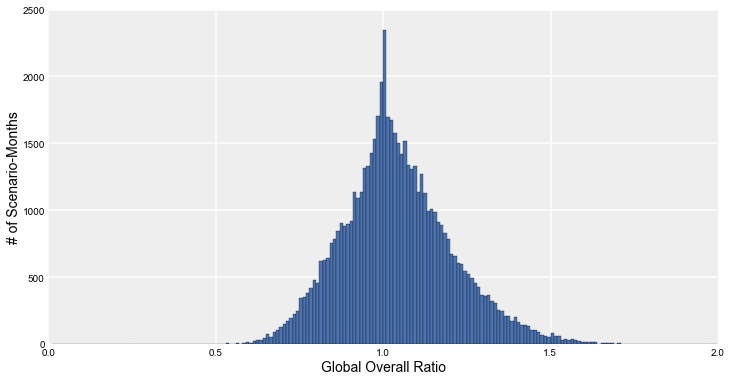
\includegraphics[width=\textwidth]{../Graphics/OverallDistribution}
	\caption{Distribution of Overall Ratios across all scenario-months}

\end{figure}

Figure 1 shows a histogram of the Global Overall Ratio (the ratio between secure demand and supply) across all iteration-months. It appears to approximate a skew normal distribution, centered very close to 1 (a balance between supply and demand) but with a longer tail to the right -- supply shocks are more likely than demand shocks, and the most extreme supply shocks the model generates, though low-probability, are more extreme than any demand shocks. 

\begin{figure}[h!]
	\centering
	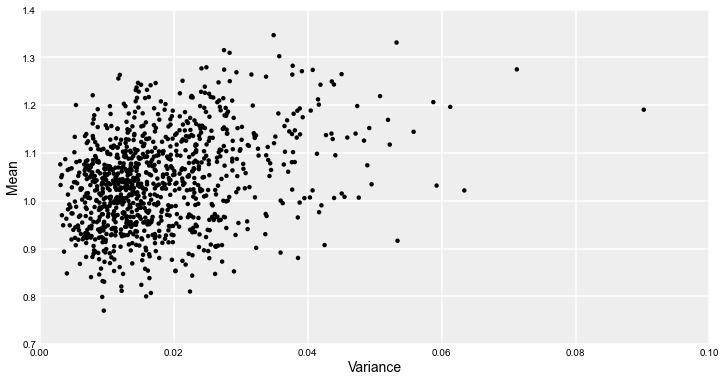
\includegraphics[width=\textwidth]{../Graphics/OverallVarMeanScatter}
	\caption{Variance and mean of Overall Ratio for each model iteration}
\end{figure}

We can also examine the model iterations separately. Initially, we can characterize each iteration by the mean and variance of each indicator, as shown in Figure 2. Note that the overall correlation between mean and variance is 0.33, indicating that they are not necessarily linearly related to one another. A high Overall or Supply mean ratio may indicate overall higher oil insecurity, but if the variance is low, it is `stably' insecure; in contrast, the mean may be close to 1 or even below it, but high variance would indicate severe uncertainty and fluctuation -- a distinct type of insecurity. 

\begin{figure}[h!]
	\centering
	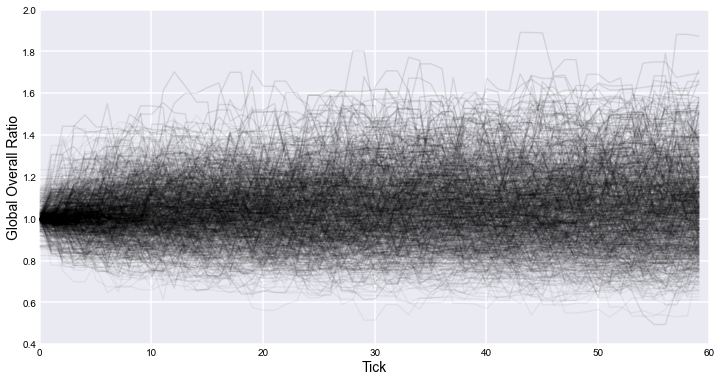
\includegraphics[width=\textwidth]{../Graphics/AllOverallTraces}
	\caption{Traces of Overall Ratio for all 1,000 iterations}
\end{figure}


We can further look at the trace of the indicators within each iteration, as they change from tick to tick. Figure 3 shows the traces of the 1,000 model runs overlaid on one another, and indicates some clear patterns. The majority of runs stay within a fairly narrow band, indicating similar levels of stability. Spikes outside the band, when they occur, tend to be brief. Note, however, that there are some longer-term plateaus and troughs -- shocks which persist for multiple months, yielding values that become at least temporary baselines, even seeing fluctuations around them.

\subsubsection{Contagion and Assistance}

In order to disaggregate the effects of the Contagion and Assistance model parameters, we examine their results separately. Figure 4 shows probability densities of the Overall Ratio for the scenario-months for Contagion and Assistance, respectively.


Upon visual examination, the distributions with Contagion enabled and disabled appear extremely similar. I conduct several statistical tests to determine whether they are in fact drawn from the same underlying distribution -- that is, whether there is no actual difference between them. Both the Kolmogorov-Smirnov  and Mann-Whitney tests indicate that the distributions are in fact different. Nevertheless, the differences are small. The mean ratio for the No Contagion scenario is 1.037, compared to 1.049 for the Contagion scenario. Both a parametric T-Test and nonparametric Wilcoxon Rank-Sum confirm that these means are indeed different, and neither the traditional (frequentist) not Bayesian confidence intervals overlap. Similarly, the variance for the No Contagion scenario is 0.025, while the Contagion variance is 0.03. Thus, conflict contagion pushes the scenarios away from the mean, yielding a wider range of outcomes. 

I repeat the same analysis for the the Assistance disabled and enabled scenarios. However, in this case, the statistical tests cannot reject the hypothesis that the resulting distributions are the same, and the means are within each other's confidence intervals.

I conduct similar analyses for the other global ratios, for supply and demand, as well, which result in the same conclusion. The effects of Contagion are small but statistically significant, while Assistance has a far smaller and less significant effect.

\subsection{Country-level analysis}

In addition to the aggregate global indicators, the model also tracks the Supply and Demand ratios for each country. We can analyze this output in order to understand how different countries' risks differ from one another, and to identify countries at high or low risk.

\begin{figure}[h!]
	\centering
	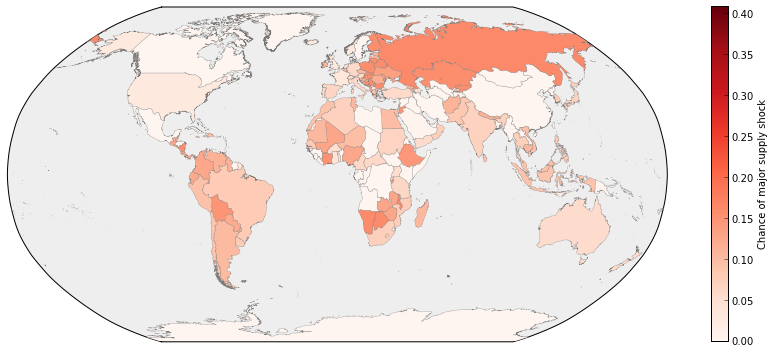
\includegraphics[width=\textwidth]{../Graphics/SupplyShockMap}
	\caption{Risk of a major supply shock (Supply Ratio $>2$)}

\end{figure}

Figure 5 shows a map of the overall risk of a major supply crisis, with the supply ratio rising above 2 (that is, demand exceeds secure supply by at least 100\%). Several things immediately jump out: major oil producers appear to be at the least risk, as their consumption of domestic production reduces their exposure to import disruption. Russia stands out as the one major producer to face a significant supply risk. The countries of the so-called `Global South' appears to face higher risks than the more developed world, likely indicating a lower diversity of import sources.

\begin{figure}[h!]
	\centering
	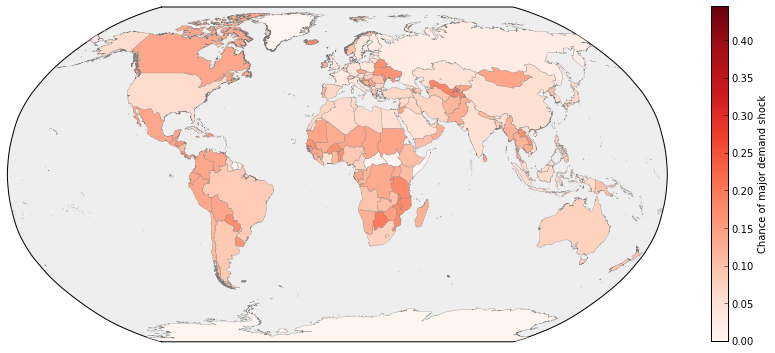
\includegraphics[width=\textwidth]{../Graphics/DemandShockMap}
	\caption{Risk of a major demand shock (Demand Ratio $<0.5$)}

\end{figure}

Figure 6 shows a similar map for demand risk, and indicates the likelihood of total possible exports exceed secure exports by at least 100\%. While there are fewer countries with very low risk, there are fewer with extremely high risk as well. Interestingly, the major Middle East producers appear to face relatively low demand risk, likely indicating a robust set of trade relationships with relatively stable countries. In contrast, the major non-US producers in the Americas -- Canada, Mexico and Venezuela -- appear to face higher demand risk. This appears to be due to the fact that their exports are disproportionately to the United States, rendering them vulnerable to US crises.

\subsection{Sensitivity Analysis}

As discussed above, the model accepts several input parameters, most of which are calibrated from data. Given that this calibration is only approximate, it is important to conduct a sensitivity analysis in order to identify whether the results are extremely sensitive to the input parameters -- the more sensitive they are, the more the model will be biased by missing or incomplete data, and the less reliable we expect it to be. The space of parameters and outputs to search is extremely large; for the purpose of this analysis, I will limit myself to two parameters: the exponential coefficient on the conflict length power law (calibrated from data, as described above) and the default spare production capacity, estimated from SME input.

In order to conduct the sensitivity analysis, I iterate over conflict coefficient values between -1.05 and -2.0, and default spare production capacities between 0 and 0.5, both in steps of 0.05. For each combination, I run the model 40 times, 10 iterations each for each combination of Contagion and Assistance, for a total of 2,200 model runs. 


Figure 7 shows the mean and variance of the Global Overall Supply and Demand Ratios produced for each iteration-tick at each combination of the parameters. Visual examination shows that there is not significant change in the Overall Ratio; the range of outputs is relatively small, and no combination of inputs produces significant outliers. The one input-output combination detectable is between the conflict coefficient and the variance. As the conflict coefficient increases (reducing the probably of long conflicts), the variance is reduced as well. However, for the Supply Ratio, there is a clear change driven by conflict coefficient: as the probability of long conflicts increases, the mean and variance increase as well (while the mean Demand Ratio, not shown, decreases). Note, however, that that there does not appear to be a clear critical point; the change is relatively linear, and the outcomes all fall within a narrow band. Note also that the calibrated value of the parameter is in the higher-variance, higher-risk zone. In other words, the model may be forecasting risk on the higher end. 



\section{Discussion}

In this paper, I have described an agent-based model to study near-future international energy security, with a focus on crude oil imports and exports. The model is data-driven, ties energy security to political crises and conflicts, and can study the effects of conflict contagion and of short-term oil production increases. We can draw two sets of conclusions from the model and its outputs: on energy security itself, as well as on the challenges of modeling it, and modeling international systems more broadly.

In terms of energy security, the model does not predict extreme shocks to be likely. Nevertheless, it shows that such extreme shocks may occur within the current configuration of the international oil system, and provides an estimate for their probability. The model indicates that consumption of domestic oil production provides a significant improvement in energy security, even in the absence of total energy independence. It also highlights the importance of diverse import and export partners. 

The model identifies the countries facing the greatest risks to their energy security, as well as making patterns in the risk visible -- particularly the high risk in the countries of the `Global South'. 

Analysis of the Contagion and Assistance parameters yields additional interesting insight. The effect of contagion is statistically significant but small -- perhaps suggesting the difficulty facing the ongoing debate over the phenomenon in political science, but also that the debate's conclusions may not be very important to policy. More counterintuitively, perhaps, the Assistance parameter does not have a significant, measurable effect. Here is somewhere the model can generate insights that are not otherwise obvious -- specifically, that even if major oil producers can rapidly increase their output in response to crises, it is not enough to counterbalance the effects of those crises. 

From a technical perspective, the model presented here is extremely simple. The interaction between agents is minimal and largely indirect, and with both Contagion and Assistance turned off, the model is essentially stochastically sampling from the space of possible crises and durations. Nevertheless, it is sufficient to capture the core aspects of the international oil system and produces useful results, demonstrating that the approach is viable. Future work can build on this framework, adding in additional submodels, dynamics and behaviors and measuring their effect against the baseline. Such additions may include explicit oil transportation and refining accounting for systemic choke-points; allowing countries to dynamically change their trading partners, supply and demand; incorporating the risks of non-political disasters both natural (e.g. Hurricane Katrina) and manmade (such as the Deepwater Horizon spill); and more.

However, as we have seen, even the simple model presented here had extensive input requirements, with data coming from various sources of varying completeness and reliability. Expanding the model would significantly increase the data requirements. Adding dynamics and behavior pose an even greater challenge. There is no complete theory of states' energy decisionmaking -- in fact, such decisionmaking is almost certainly embedded within a broader policy framework, tied to both external interests and internal issues. It may be the case that adding additional elements will make the model more brittle without adding validity or increasing predictive power.

Finally, the model presented here may have another application, as a decision-support tool for policymakers. The model's user interface (both via input files and a GUI) allows specific scenarios to be initiated and run, and their consequences and outputs evaluated. This may range from simply testing the effect of a particular events (e.g. a 12-month internal crisis in Saudi Arabia) to estimating the broader consequences of structural change (what would be the consequences if China were to become 10\% less stable, or if Iran were to begin to export to Europe). By quickly setting up and observing a `state of the world', a policymaker can augment her intuition, test hypotheses, and identify interesting issues or outliers for further qualitative or quantitative analysis. 

\bibliographystyle{splncs}
\bibliography{energysecurity}

\end{document}